\subsection{Pipeline overview}\label{subsec:knowledge-pipeline-overview}

The pipeline consists of seven stages, where each stage consumes the typed object the previous stage produced. The flow is mostly linear, except at the end: the RELATE stage computes the pairwise relations of the canonical rules, making RESOLVE the only stage that consumes two inputs --- the canonical rules from CANONICALIZE and the relations from RELATE, which it uses to score each rule. Figure~\ref{fig:ke-pipeline} shows these stages with their per-stage input and output types. 

\begin{figure}[htbp]
    \centering
    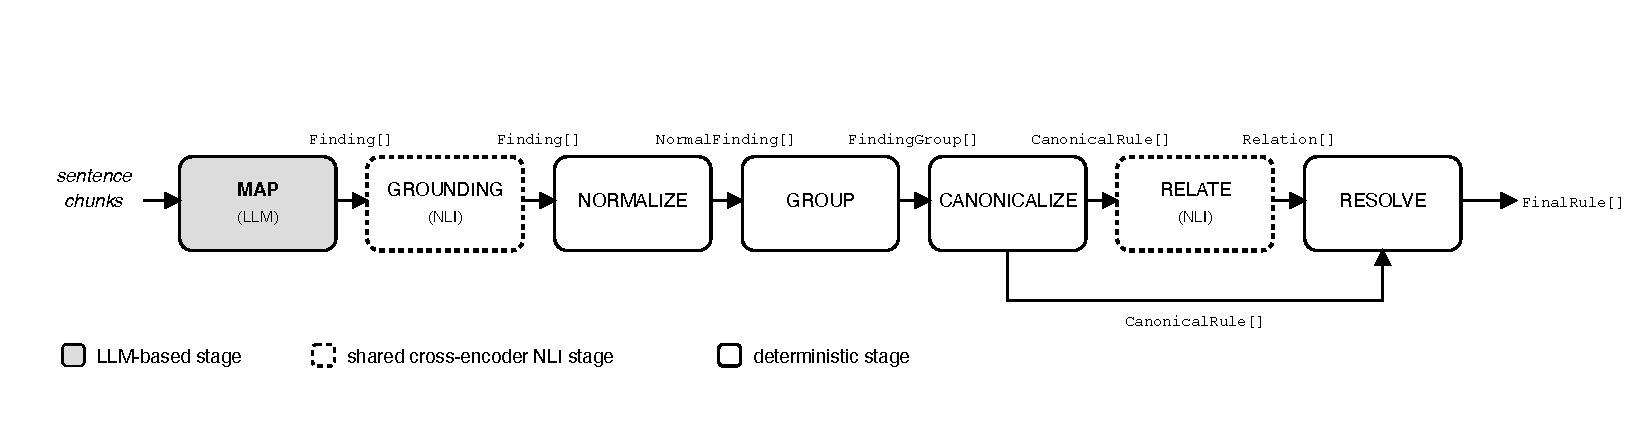
\includegraphics[width=\textwidth]{figures/03_methodology/04_knowledge_extraction/01_knowledge_pipeline.pdf}
    \caption{Knowledge-extraction pipeline, with each arrow labelled by the typed object it emits. GROUNDING is a filter, so it preserves the type; RESOLVE takes multiple inputs.}
    \label{fig:ke-pipeline}
\end{figure}

The input is a list of source sentence chunks for each paper. Each sentence has the stable database identifier of the paragraph it was segmented from. The output is a list of \texttt{FinalRule} records, which are typed, ranked, and traceable back to their source texts; and a separate list of \texttt{Relation} records, which describe the links between the rules.

MAP is the only stage that calls a large language model; it converts input chunks to typed candidate findings. Two later stages, GROUNDING and RELATE, share a single cross-encoder NLI model: GROUNDING discards findings whose verbatim support does not entail the claim, and RELATE classifies the relationship between canonical rules. The remaining four stages are deterministic: NORMALIZE resolves entities using a fixed UMLS-supported linker, GROUP clusters compatible findings, CANONICALIZE converts grouped findings into rule candidates, and RESOLVE assigns the final rule scores. Confining the stochastic part of the system to a single MAP stage makes the cost-quality calibration of MAP, described in Section~\ref{section:Agreement_Based_Cascading}, a self-contained engineering problem. 